\section{Results}
\label{sec:results}

\subsection{Raw Transfer Function Data}
\label{sec:raw-data}

\Cref{fig:raw-H} shows the measured transfer function magnitude $|H(x)|$ at
$f = \SI{0.1}{\hertz}$ as a function of distance. The data exhibits a smooth,
monotonically decreasing trend from $|H| = 0.161$ at $x = \SI{10}{\um}$ to
$|H| = 0.039$ at $x = \SI{2000}{\um}$, representing a dynamic range of
approximately 4:1.

Below \SI{200}{\hertz}, the transfer function magnitudes are virtually
independent of frequency, consistent with the quasi-static behavior expected
from the magnetic circuit at low frequencies. Above \SI{200}{\hertz}, the
magnitudes decrease due to the second-order dynamics of the
actuator~\cite{Zhang2010}.

\begin{figure}[htbp]
\centering
\includegraphics[width=0.7\textwidth]{../results/Charge_NTU/figures/Charge_Fit_Single_0p1Hz.png}
\caption{Transfer function magnitude $|H(x)|$ at $f = \SI{0.1}{\hertz}$
with the inverse-square model fit. Data (circles) and model
$H = a^2/(x+b)^2$ (solid line) with $b = \SI{1979}{\um}$.}
\label{fig:raw-H}
\end{figure}

\subsection{Inverse-Square Fitting}
\label{sec:fitting}

The model $H(x) = a^2 / (x+b)^2$ is fitted independently at each of three
low frequencies ($0.1$, $1$, and $\SI{10}{\hertz}$) where the system is
quasi-static. The results are summarized in \cref{tab:fit-results}.

% Table 2: Inverse-square fitting results
% Data from Charge_Fit_Results.csv (Charge_NTU)
\begin{table}[htbp]
\centering
\caption{Inverse-square fitting results at three frequencies. The model
$H(x) = a^2/(x+b)^2$ is linearized as $1/\sqrt{H} = x/a + b/a$ and
fit by least-squares regression.}
\label{tab:fit-results}
\begin{tabular}{@{}lccc@{}}
\toprule
Frequency (Hz) & $a$ & $b$ (\si{\um}) & $R^2$ \\
\midrule
0.1  & 765.57 & 1979.3 & 0.9921 \\
1    & 764.84 & 1977.6 & 0.9921 \\
10   & 765.63 & 1979.9 & 0.9919 \\
\midrule
Mean $\pm$ Std & $765.35 \pm 0.43$ & $1978.9 \pm 1.2$ & --- \\
\bottomrule
\end{tabular}
\end{table}


The key findings are:
\begin{itemize}
\item The offset $b = 1978.9 \pm \SI{1.2}{\um}$ is consistent across all
three frequencies, confirming that $b$ is a geometric property of the magnetic
circuit independent of excitation frequency.
\item The coefficient of variation of $a$ is $\mathrm{CV} = 0.06\%$,
indicating excellent measurement reproducibility.
\item $R^2 > 0.991$ for all fits, demonstrating that the inverse-square model
captures the dominant behavior.
\end{itemize}

\Cref{fig:overlay} shows the three fitted curves overlaid on the data,
and \cref{fig:summary} shows the consistency of $b$ and $R^2$ across
frequencies.

\begin{figure}[htbp]
\centering
\includegraphics[width=0.7\textwidth]{../results/Charge_NTU/figures/Charge_Fit_Overlay.png}
\caption{Inverse-square fits at three frequencies overlaid on measured data.
All three curves are virtually indistinguishable, confirming frequency
independence.}
\label{fig:overlay}
\end{figure}

\begin{figure}[htbp]
\centering
\includegraphics[width=0.7\textwidth]{../results/Charge_NTU/figures/Charge_Fit_Summary.png}
\caption{Fitting consistency. Top: $b$ vs.\ frequency with mean and
$\pm 1\sigma$ band. Bottom: $R^2$ vs.\ frequency.}
\label{fig:summary}
\end{figure}

The linearized representation $1/\sqrt{H}$ vs.\ $x$ (\cref{fig:linearized})
provides visual confirmation that the data follows a straight line, as
predicted by \cref{eq:linearized}. The residuals show no systematic trend,
indicating that higher-order multipole terms are negligible over the measured
distance range.

\begin{figure}[htbp]
\centering
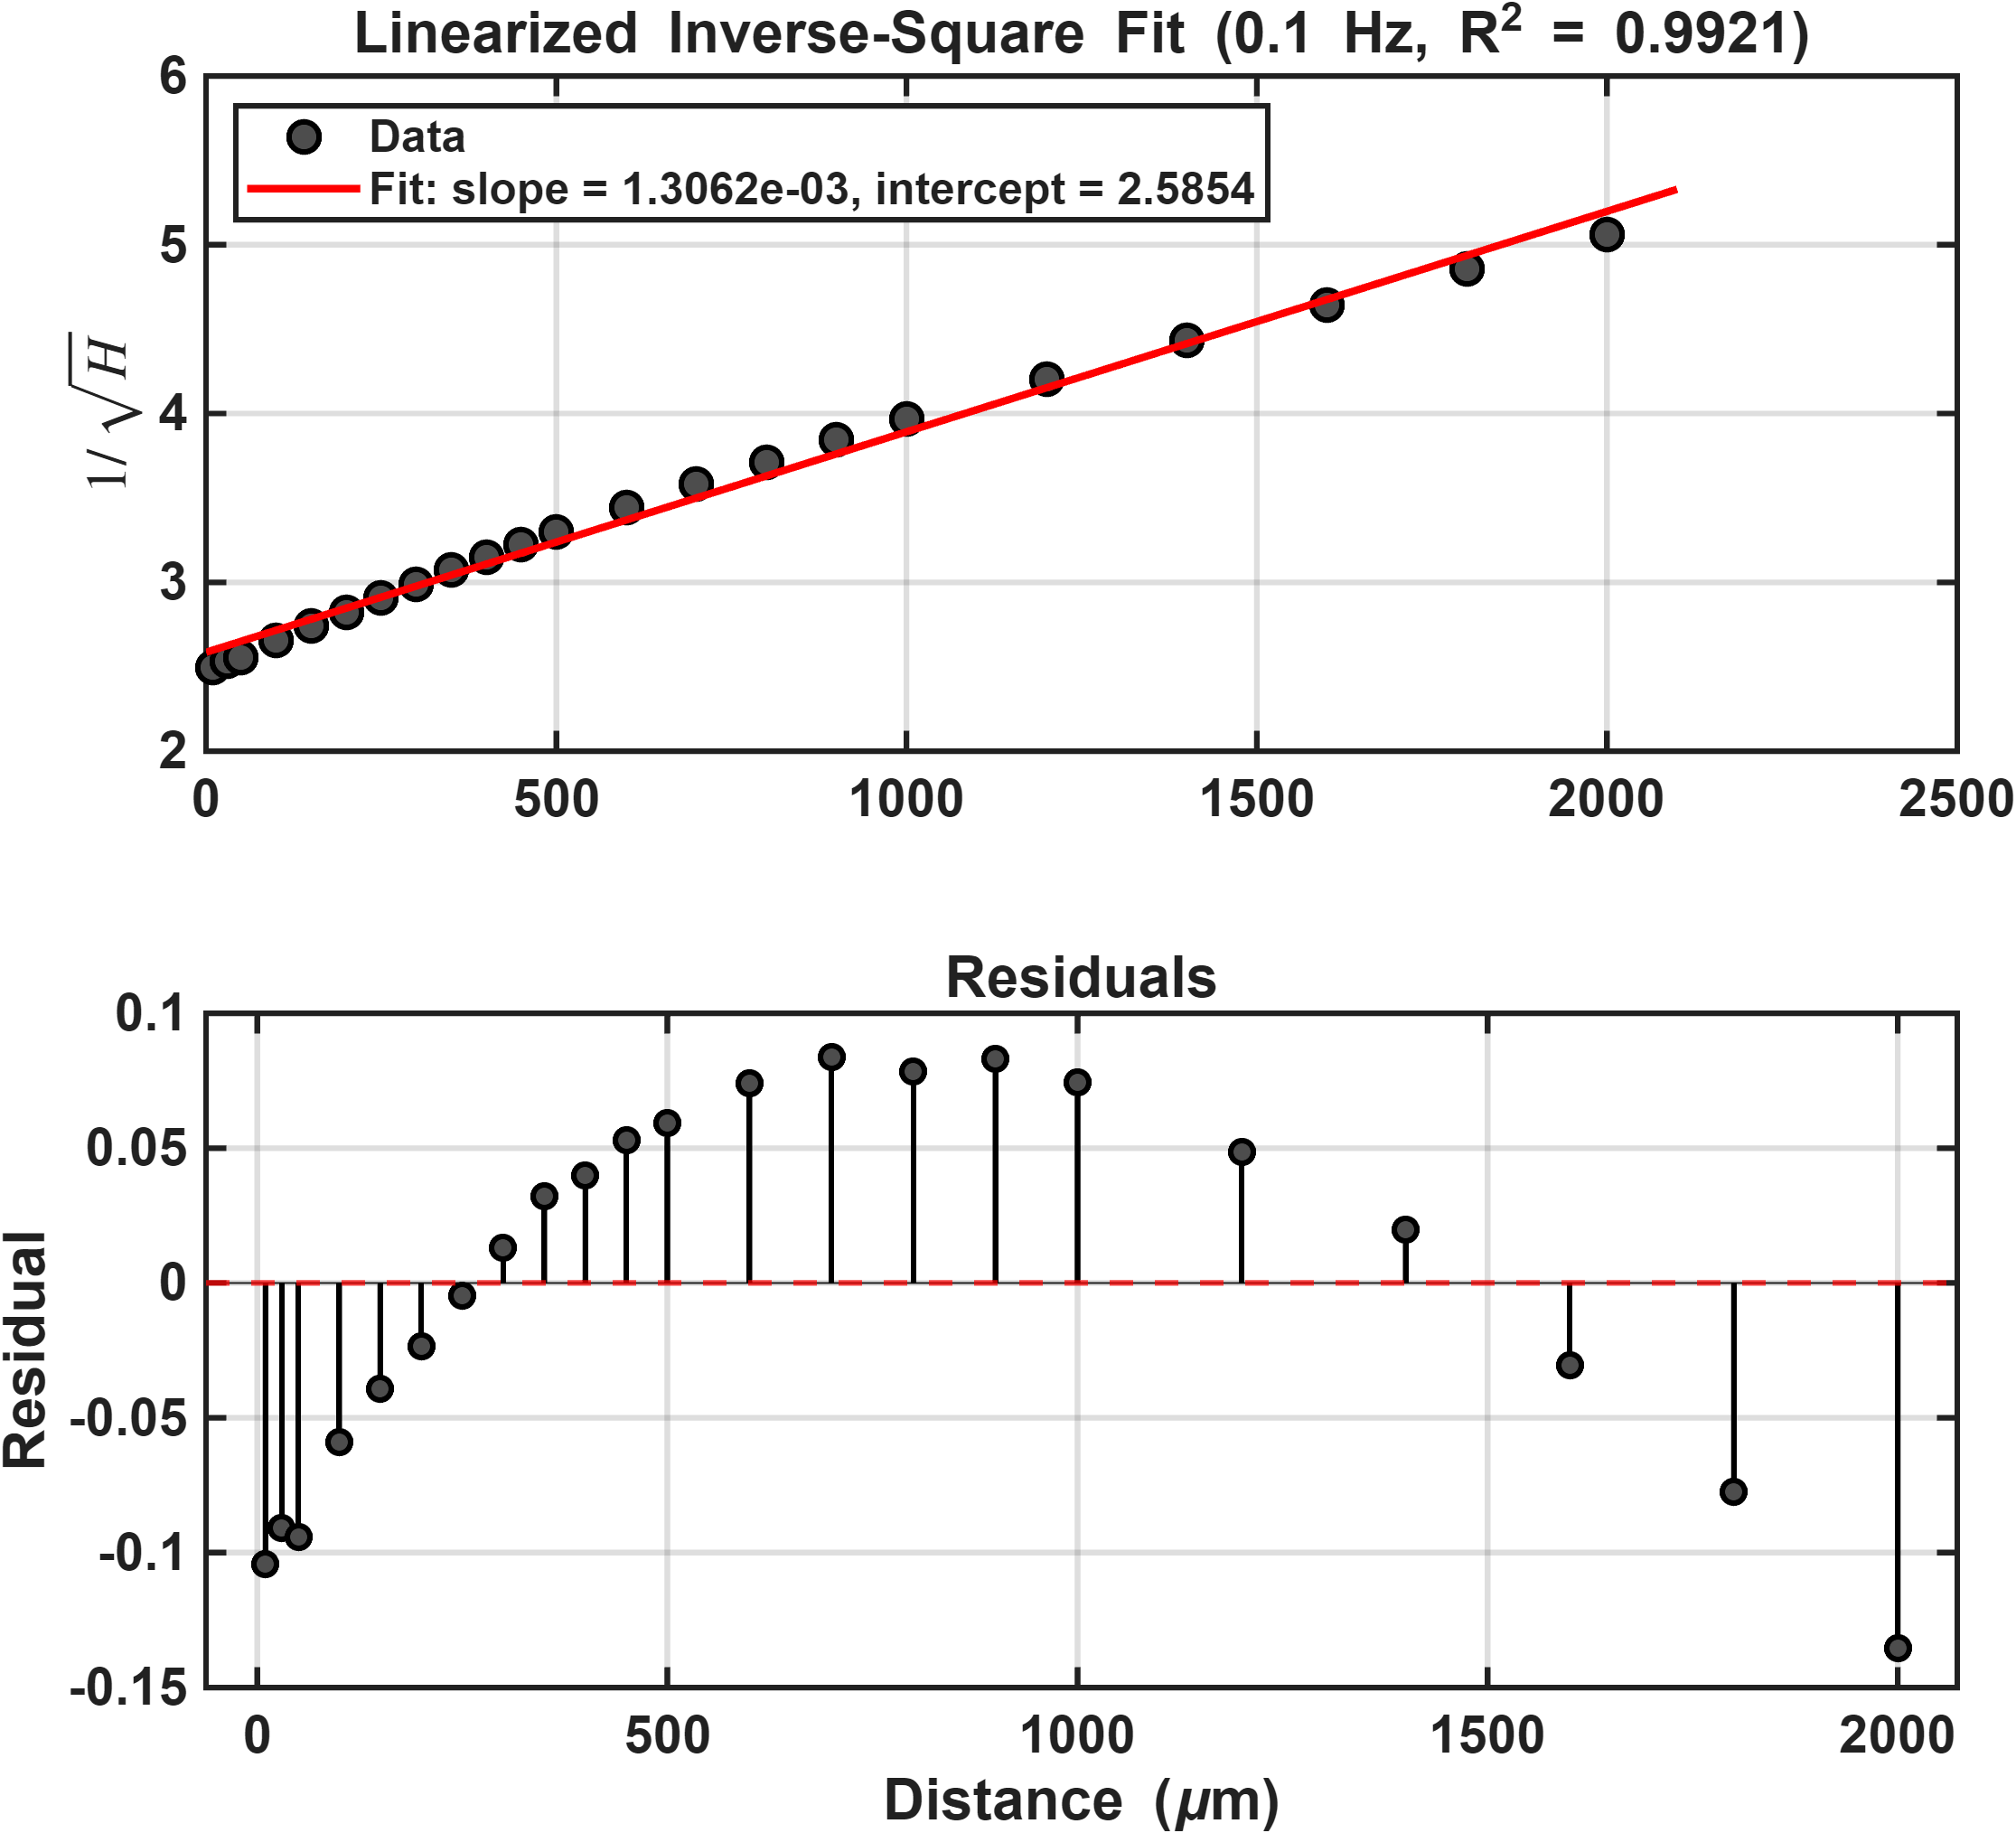
\includegraphics[width=0.7\textwidth]{figures/linearized_fit.png}
\caption{Linearized fit at $f = \SI{0.1}{\hertz}$. Top: $1/\sqrt{H}$ vs.\
distance with linear regression. Bottom: residuals.}
\label{fig:linearized}
\end{figure}

\subsection{Distance Range Sensitivity}
\label{sec:range-sensitivity}

The fitted value of $b$ depends on the distance range included in the fit.
When the fit is restricted to $x \in [10, 500] \;\si{\um}$, the result is
$b \approx \SI{1504}{\um}$, compared to $b = \SI{1979}{\um}$ for the full
range $x \in [10, 2000] \;\si{\um}$.

This behavior is expected: the pure inverse-square (monopole) model is an
approximation, and at short distances, higher-order multipole contributions
become relatively more significant. Fitting over a wider range of distances
provides a more robust estimate of the effective monopole offset.

\begin{figure}[htbp]
\centering
\includegraphics[width=0.7\textwidth]{../results/Charge_NTU/figures/Charge_Fit_Single_0p1Hz_10to500um.png}
\caption{Inverse-square fit restricted to $x \in [10, 500]\;\si{\um}$,
yielding $b \approx \SI{1504}{\um}$. The shorter range gives a smaller $b$
due to unmodeled multipole contributions at close distances.}
\label{fig:short-range}
\end{figure}
